In the tau reconstruction, $\tauhad$ candidates are seeded from jets. Therefore, QCD events represent the main source of background (BG). Nonetheless, we do not have MC simulations for this processes. For this reason, we use a \textit{data driven method} to estimate multi-jet (MJ) BG. On the other hand, the main electroweak background (EWBG) contribution will come from $\Wjets$ production, where the light-lepton comes from the W decay and one jet fakes the $\tauhad$. In this section we will discuss how we derived our BG estimation.

\subsection{Multi-Jet Background}
To obtain the multi-jet background (MJBG), a variable that in principle is supposed to be uncorrelated with the shape of the MJBG is chosen. For our study, this variable is the relative sign between the charges of the $\tauhad$ and the lepton. This defines two regions: the same sign (SS) region where $q(\tauhad)=q(l)$ and the opposite sign region where $q(\tauhad)=-q(l)$. Our estimate for the MJBG in the SS region is obtained by subtracting signal and electroweak backgrounds (EWBG) contributions:
\begin{equation}
\text{MJBG}_{\text{SS}}=\text{Data}_{\text{SS}}-\text{Signal}_{\text{SS}}-\text{EWBG}_{\text{SS}},
\label{eq19}
\end{equation}
 To study the residual charge correlation, we define a control region (CR) where the MJ background is enhanced. The estimate for the MJBG in these regions is given by eq. \ref{eq19} as well. The region described in Sec.\ref{sec3.3}, which contains all our final selected events is called the signal region (SR). In contrast to the SR, the CR is defined by events that fail the lepton isolation criteria and that fail the Tight-ID working point criterion for the $\tauhad$ candidate. The other kinematic features of the SR are maintained. A diagram showing the four regions just defined is shown in Fig.\ref{Fig7}. Now, if we assume that charge correlation is the same in the SR and CR, we have:
 \begin{equation}
 \frac{\text{MJBG}_{\text{SR OS}}}{\text{MJBG}_{\text{SR SS}}}=\frac{\text{MJBG}_{\text{CR OS}}}{\text{MJBG}_{\text{CR SS}}},
 \end{equation}
then,
 \begin{equation}
\text{MJBG}_{\text{SR OS}}=\text{MJBG}_{\text{SR SS}}\times \text{RQCD}\,
\label{eq36}
\end{equation}
where $\text{RQCD}\equiv\frac{\text{MJBG}_{\text{CR OS}}}{\text{MJBG}_{\text{CR SS}}}$. So, \eqref{eq36} gives the estimation of MJBG on the SROS.
\begin{figure}[htbp]
	\centering
	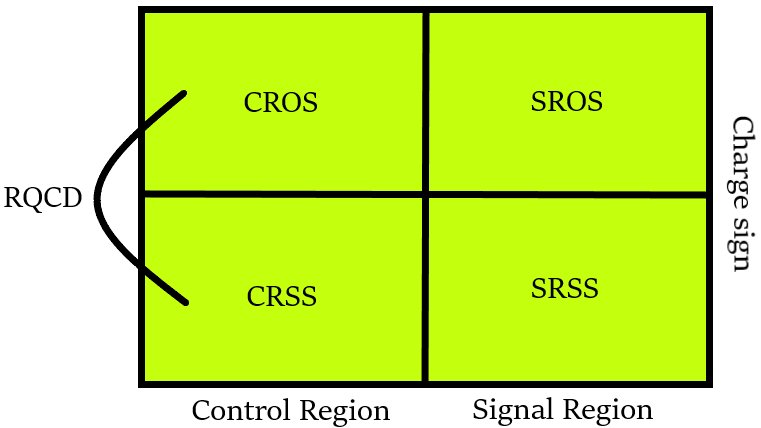
\includegraphics[width=0.5\textwidth]{figures/Fig7.png}
	\caption{Regions defined to estimate MJ background contribution in the SROS region. This data-driven method is also known as the ABCD method.}
	\label{Fig7}
\end{figure}
Table \ref{tab:MJ} summarises inputs into the calculation of the MJ background in the three candidate event samples. 
\begin{table}[]
	\resizebox{\textwidth}{!}{%
		\begin{tabular}{ccccc}
			\rowcolor[HTML]{C0C0C0} 
			\textbf{Sample} & \multicolumn{2}{c}{\cellcolor[HTML]{C0C0C0}\textbf{$\mu \tauhad$}} & \multicolumn{2}{c}{\cellcolor[HTML]{C0C0C0}\textbf{$e \tauhad$}} \\
			& 1-prong                                  & 3-prong                                 & 1-prong                                 & 3-prong                                \\ \hline
			CR OS Data      & 1696.0                                   & 914.0                                 & 323.0                                  & 188.0                                 \\
			MC              & 120.865                                 & 35.63                                & 49.943                                & 19.197                                \\
			CR SS Data      & 1394.0                                   & 647.0                                   & 307.0                                  & 111.0                                  \\
			MC              & 30.428                                  & 4.339                                  & 21.698                                 & 2.584                                 \\ \hline
			RQCD            & 1.155                                    & 1.367                                   & 0.957                                   & 1.557                                  \\ \hline
			SR SS Data      & 215.0                                    & 30.0                                    & 212.0                                   & 30.0                                   \\
			MC              & 132.227                                  & 8.06                                    & 135.354                                 & 33.774                                 \\ \hline
			MJ Background   & 95.615                                  & 29.986                                  & 73.356                                 & 0.0                                   
		\end{tabular}%
	\caption{Inputs for the calculation of the MJBG in the two final states, $Z\to\mu\tauhad$ and $Z\to e\tauhad$.
		The numbers of data events in the CR OS and CR SS samples are given, together with the total numbers of events in these
		categories expected from simulation.
		The excess of data with respect to simulation is assumed to arise from MJBG and it is used to calculate the value of RQCD.
		The quoted uncertainties are statistical only.
	}

	\label{tab:MJ}
}
\end{table}

\subsection{Electroweak Background}
As we discussed previously, the main source of EWBG comes from $\Wjets$ events. Other sources of EWBG are $t\bar{t}$, $\Zjets$, Diboson and single top processes. For all of them, simulated samples are available and they are listed in Table \ref{Table3}. In order to check if the $\Wjets$  simulation is correctly accounting for the expected EWBG, we define a CR where there is an enhanced fraction of expected $\Wjets$ events. In this region, we require our events to lay in the $\Omega<0$ or $\Omega>1.4$ bands. We also make a requirement in transverse mass of the lepton, $M_T(l)\ge 60 \GeV$. Finally, we require $n_{\text{jets}}\le 2$ to reduce $t\bar{t}$ BG. The other selections of our SR are kept.

To evaluate the MJBG contribution in the $\Wjets$ CR we use the ABCD method. Our CR for MJBG is defined by the events that fail the light-lepton isolation or that have a $\tauhad$ candidate with more than 15 total tracks (CHANGE?). The  $M_T(l)$ distribution for our $\Wjets$ events is shown in Fig.\ref{Fig8}. 
\begin{figure}[htbp]
	\centering
	\subfloat[]{\label{Fig8a}{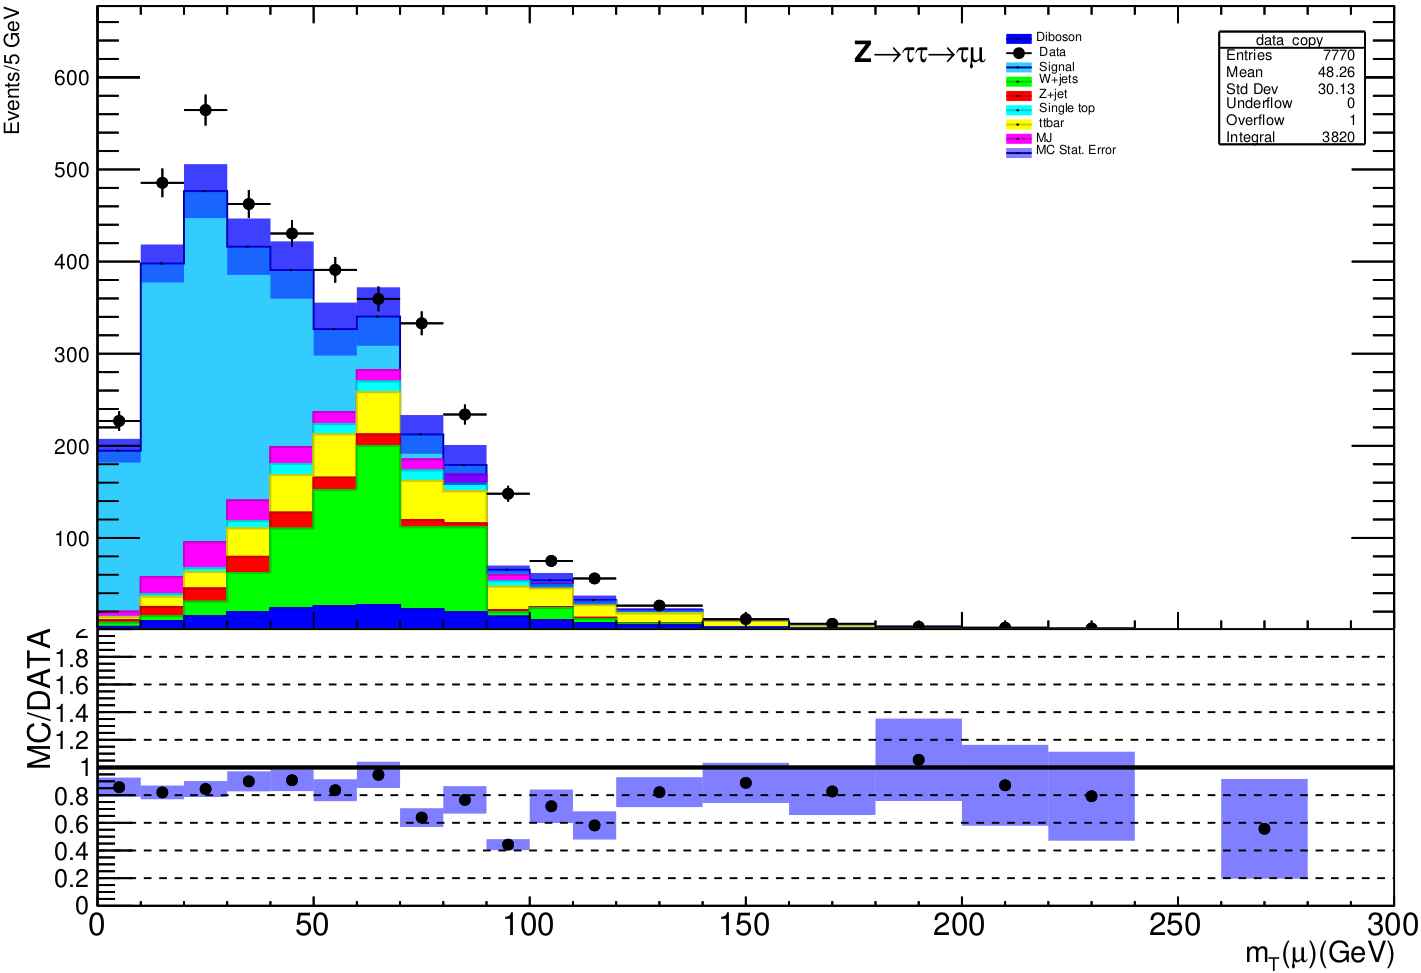
\includegraphics[width=0.50\textwidth]{figures/Fig8a}}}\hfill
	\subfloat[]{\label{Fig8b}{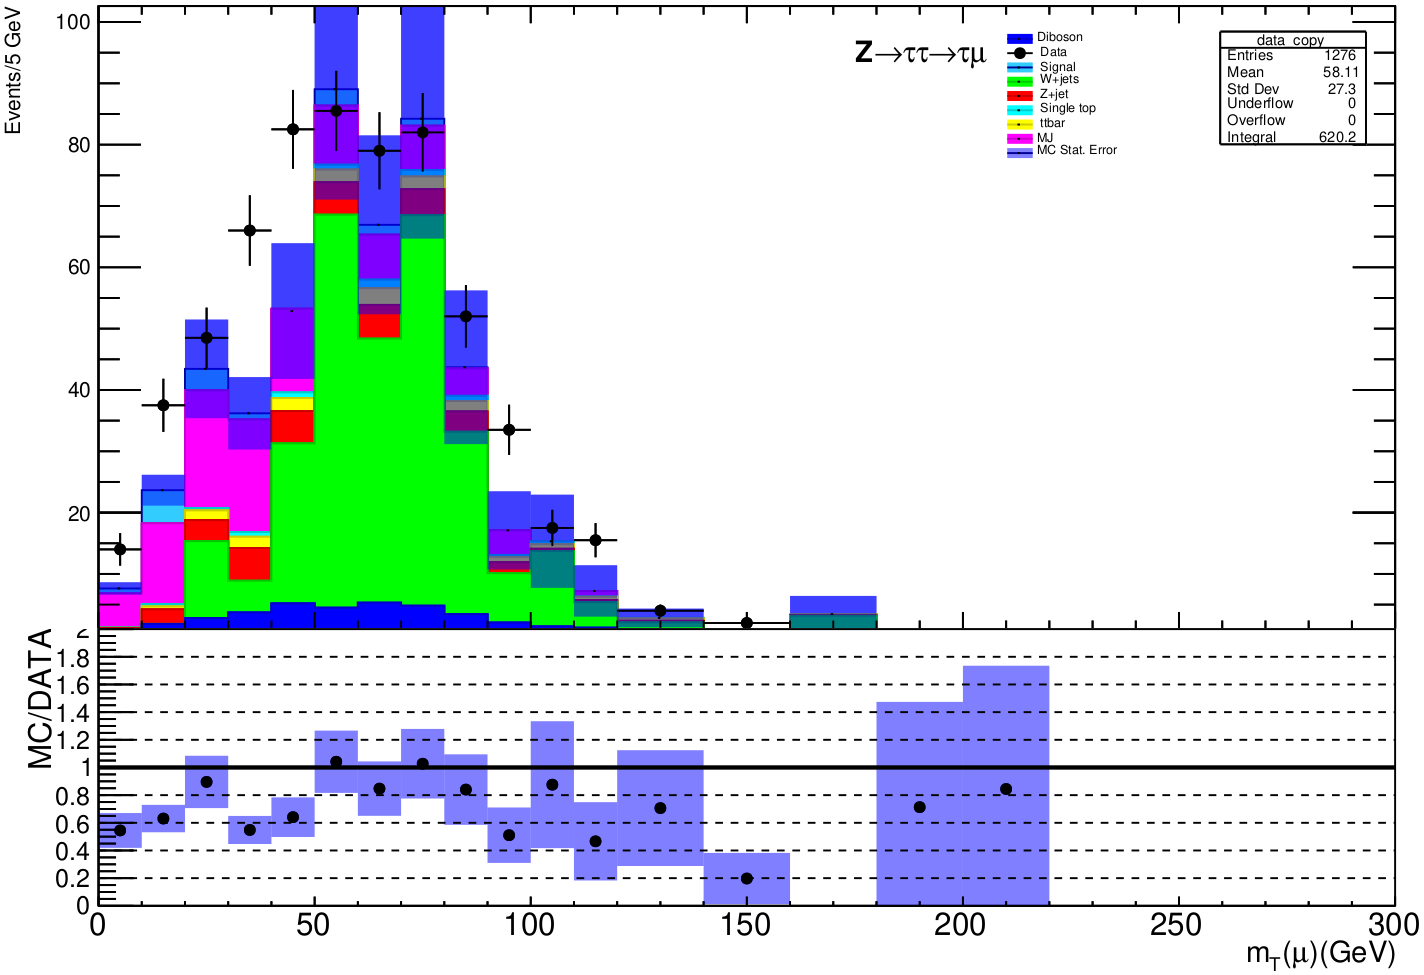
\includegraphics[width=0.50\textwidth]{figures/Fig8b}}}
	\caption{$M_T(l)$ distribution for the OS (a) and SS (b) regions. All the other cuts have been applied apart from the one being plotted. There is an excess of the data in this distribution which suggest that the simulation could be underestimating the number of $\Wjets$ events.}
	\label{Fig8}
\end{figure} 
The plots show that the simulation is in average below the observed events. For this reason, in this analysis we have taken a conservative approach and had scaled up our $\Wjets$ yields in the SR by a factor of 0.8$\pm$0.2 .